%!TEX root = ..\..\main.tex
\chapter{Deconvolution}
\label{Ch:Deconvolution}

\lhead{Chapter \ref{Ch:Deconvolution}. \emph{Deconvolution}}

%-------------------------------------------------------------------------------
%	Chapter Text
%-------------------------------------------------------------------------------

% Quick summary of what Aurore said she expected the chapter to contain
% Explain basic deconvolution, phiU known
% PhiU est from replicates
% With no replicates brief summary of lit
% Delaigle Hall 2016
% Say authors noted few points of support
% Hard to come up with theoretical justification for why
% Here's empirical examples
% Looks like often need a lot less
% Motivates code with fewer parameters. This is faster.
% We do this in R-package.

\section{Introduction}
	In this final chapter, we look at another statistical problem in which we perform an optimization over discrete probability distributions and find that the number of points of support of the optimal distribution is much smaller than expected. In contrast to Chapter \ref{Ch:Mixtures}, we will take a descriptive and practically minded point of view, rather than the more theory driven previous chapter. This is partly due to the additional complexity of the problem, which prevents many of the tools used on maximum likelihood mixtures from working here. However, this does not stop us from pointing out many similarities between the two problems, and an empirical exploration allows us to benefit from the similar phenomenon that occurs in a variety of scenarios.

	The problem is one of \emph{deconvolution}, the recovery of the distribution, $F_X$, or density, $f_X$, of some random variable $X$, from measurements of
	\begin{equation}
		W = X + U
	\end{equation}
	where the measurement error $U$ is independent of $X$. 

	In the case that we know the distribution of $U$, Carroll and Hall \cite{Carroll1988-aj} and Carroll and Stefanski \cite{Stefanski1990-uo} proposed a deconvolution kernel density estimator of $f_X$. If the distribution of $U$ is unknown, then we may hope to estimate it from replicate measurements, $W_{jk} = X_j + U_{jk}$, for $1 \leq k \leq N_j$ and $1 \leq j \leq n$. Delaigle, Hall, and Meister provide an estimator for $f_X$ in this scenario. However, up until Delaigle's and Hall's 2016 paper, ``Methodology for nonparametric deconvolution when the error distribution is unknown,'' \cite{Delaigle2016-la}, there had been no nonparametric method to estimate the distribution of $X$ when we had no data on the distribution of $U$ (see the discussion in Section 1 of \cite{Delaigle2016-la}).

	% [BRIEF SUMMARY OF LITERATURE]

	In this chapter, we focus on the methods introduced in this paper. We will start in Section \ref{sec:summary of basic deconvolution} by summarizing deconvolution methods for when the error distribution is known, or estimated from replicates. This will serve as a basis for a discussion on Delaigle's and Hall's ``Methodology for nonparametric deconvolution when the error distribution is unknown,'' in Section \ref{sec:summary of delaigle hall}. In Section \ref{sec:deconvolution empirical results}, we will empirically demonstrate that these methods produce a similar phenomenon to the one encountered when using maximum likelihood location mixtures, and we will explore how this phenomenon manifests under various conditions. We will also point out how we can take advantage of this phenomenon. Finally, in Section \ref{sec:deconvolution observations and results}, we will make some general observations about some similarities between our deconvolution problem, and that of maximum likelihood mixtures. 

\subsection{Prior deconvolution methods}
\label{sec:summary of basic deconvolution}
% \subsection{PhiU known}
	We start with the estimator of Stefanski and Carroll in \cite{Stefanski1990-uo}. In this scenario, we let $X$ and $U$ be independent random variables with probability density functions $f_X$ and $f_U$ respectively. We observe a set of n independent observations, $\{W_j\}_{j = 1}^n$, where each $W_j$ is an observation of 
	\begin{equation}
		W = X + U.
	\end{equation}
	Furthermore, we assume that $f_U$ is known. Given this information, the goal is to estimate $f_X$.

	The estimator makes use of characteristic functions. A random variable $X$ with density $f_X$ has characteristic function
	\begin{equation}
		\phi_X(t) = \int \euler^{i t x} f_X(x) \intd x
	\end{equation}
	which can be inverted via
	\begin{equation}
		f_X(x) = \frac{1}{2\pi} \int \euler^{-itx} \phi_X(t) \intd t
	\end{equation}
	if $\phi_X$ is integrable. One property of characteristic functions that is convenient for this deconvolution problem is that since $X$ and $U$ are independent, we know that the characteristic function of $W = X+ U$ is
	\begin{equation}
		\phi_W = \phi_X \phi_U,
	\end{equation}
	or equivalently,
	\begin{equation}
		\phi_X = \frac{\phi_W}{\phi_U}
		\label{eq: phi_X is fraction phi_W phi_U}
	\end{equation}
	if $|\phi_U(t)| > 0$ for all real $t$. We assume this in the following estimator.

	Let $f_K$ be a bounded, even, probability density function whose characteristic function, $\phi_K$, satisfies
	\begin{align}
		\sup_t |\phi_K(t) / \phi_U(t / h) | < \infty, &&\int|\phi_K(t) / \phi_U(t / h)| \intd t < \infty,
	\end{align}
	for any fixed $h > 0$ (we impose these conditions make various functions integrable). We may estimate the density of $W$ via the usual kernel density estimator
	\begin{equation}
		\hat{f}_W(t) = \frac{1}{n h} \sum_{j = 1}^n K((W_j - x)/h),
	\end{equation}
	which has characteristic function
	\begin{equation}
		\hat{\phi}_W(t) = \phi_{W_\mathrm{EMP}}(t) \phi_K(h t)
	\end{equation}
	where $\phi_{W_\mathrm{EMP}}(t)$ denotes the empirical characteristic function of $\{W_j\}_{j = 1}^n$,
	\begin{equation}
		\phi_{W_\mathrm{EMP}}(t) = \frac{1}{n}\sum_{j = 1}^n \euler^{itW_j}.
	\end{equation}

	Motivated by \eqref{eq: phi_X is fraction phi_W phi_U}, we may estimate the characteristic function of $X$ by 
	\begin{equation}
		\hat{\phi}_X = \hat{\phi}_W / \phi_U
	\end{equation}
	and the density of $X$ by inverting $\hat{\phi}_X$. Overall, the estimator for $f_X$ is given by
	\begin{equation}
	\label{eq:standard deconvolution estimator}
		\hat{f}_X(x) = \frac{1}{2\pi} \int \euler^{-itx} \phi_K(ht) \phi_{W_\mathrm{EMP}}(t)  / \phi_U(t) \intd t.
	\end{equation}

% \subsection{PhiU est from replicates}
	If the distribution of $U$ is unknown, we may still be able to estimate it if replicate measurements are present. Methods for deconvolution with the presence of replicates are presented in \cite{Li1998-mj}, \cite{Lin2006-mm}, \cite{Delaigle2008-hl}, and also \cite{McIntyre2011-fg} in the case of heteroscedastic errors. Here we look at the estimator of Delaigle, Hall, and Meister \cite{Delaigle2008-hl} as it has the most similarities with the estimator of interest in this chapter.

	In this setting, we measure
	\begin{align}
		W_{jk} = X_j + U_j && j = 1, \dots, n \text{ and } k = 1, \dots, N_j
	\end{align}
	where the $X_j$ and $U_{jk}$ are independent and are identically distributed as $X$ and $U$ respectively. A consistent estimator of $\phi_U$ is
	\begin{equation}
		\hat{\phi}_U(t) = \left|\frac{1}{N} \sum_{j = 1}^n \sum_{(k1, k2) \in \mathscr{S}_j} \cos \left(t (W_{jk_1} - W_{jk_2}\right)\right|^{1/2}.
	\end{equation}
	In light of \eqref{eq:standard deconvolution estimator}, this suggests an estimator of $f_X$ given by 
	\begin{equation}
	\label{eq:replicates estimator}
		\hat{f}_X(x) = \frac{1}{2\pi} \int \euler^{-itx} \phi_K(ht) \phi_{W_\mathrm{EMP}}(t)  / (\hat{\phi}_U(t) + \rho )\intd t
	\end{equation}
	with
	\begin{equation}
		\phi_{W_\mathrm{EMP}}(t) = \frac{1}{M} \sum_{j = 1}^n \sum_{k= 1}^{N_j} \euler^{i t W_{jk}}
	\end{equation}
	where
	% \begin{equation}
	% 	\hat{f}_X(x) = \frac{1}{Mh} \sum_{j = 1}^n \sum_{k = 1}^{N_j} \hat{L}\left(\frac{x - W_{jk}}{h}\right)
	% \end{equation}
	% where
	% \begin{equation}
	% 	\hat{L}\left(u\right) = \frac{1}{2\pi} \int \euler^{-itu} \phi_K(t) / (\hat{\phi}_U(t/h) + \rho) \intd t,
	% \end{equation}
	$h > 0$ is a bandwidth, $\rho \geq 0$ is a ridge parameter, and $K$ is a symmetric kernel density with compact support, whose characteristic function, $\phi_K$, has compact support.

	[WHY COMPACT SUPPORT?]

	The presence of the ridge parameter is to account for potential fluctuations in $\hat{\phi}_U$ that could cause the denominator in \eqref{eq:replicates estimator} to be zero, or too close to zero. We may alternatively use another method to prevent $\hat{\phi}_U$ from getting too close to zero such as replacing $\hat{\phi}_U(t)$ with some other function for $|t|$ larger than some threshold $t^*$.

	A similar approach could be used in scenarios where we are able to sample directly from the distribution of $U$. See also \cite{Diggle1993-jy} and \cite{Neumann1997-cr} for further discussion of cases where samples of the errors are available.

	% \subsection{U unknown}
	In the case where we do not know the distribution of $U$, nor have access to replicate measurements or direct measurements from $U$, methods for deconvolution generally require $F_U$ to have a parameteric or semi-parametric form. Such methods can be found in \cite{Butucea2005-be}, \cite{Meister2006-nu}, \cite{Butucea2008-wm}, and \cite{Kneip2012-aa}.
 
\section{Method for deconvolution when the error is unknown}
\label{sec:summary of delaigle hall}
	Delaigle's and Hall's 2016 paper, ``Methodology for nonparametric deconvolution when the error distribution is unknown,'' \cite{Delaigle2016-la}, presents a non-parametric deconvolution estimator for when the error distribution is unknown, and we do not have access to replicates or samples from the error distribution. This is unusual in deconvolution problems. As in the methods described above, deconvolution methods usually require assumptions about the shape or scale of the error distribution, or rely on additional samples to estimate it. 

	In this section we summarise the estimator of \cite{Delaigle2016-la}, and discuss some practicalities that arise in the implementation. 

	\subsection{Problem Setup}
	Suppose that we have $n$ observations of
	\begin{align}
		W_j &= X_j + U_j &&j = 1, \dots, n
	\end{align}
	where $X_j$ and $U_j$ are independent and identically distributed as $X$ and $U$ respectively, and $X$ and $U$ are independent. We use $\phi_X$ and $\phi_U$ to denote the characteristics functions of $X$ and $U$, and $F_X$ and $F_U$ for the distributions. We use $f_X$ and $f_U$ for the densities if they exist.

	% Suppose also that we do not know any information concerning the distribution of $U$. This is unusual in deconvolution problems; we usually assume that we either know the distribution of $U$, at least up to a scaling factor, or that replicate measurements of the $W_j$s are available for the same $X_j$. 

	We still make some assumptions about $U$ and its characteristic function, $\phi_U$. These are 
	\begin{assumption}
	\label{assump:phiU real}
		$\phi_U$ is real-valued.
	\end{assumption}
	\begin{assumption}
	\label{assump:phiU non zero}
		For $U$ discrete, $\phi_U$ is non-negative and is zero at at most a countable number of points, and for $U$ continuous, $\phi_U$ is strictly positive on the whole real line.
	\end{assumption}

	Assumption \ref{assump:phiU real} is equivalent to assuming that $F_U$ is symmetric. Assumption \ref{assump:phiU non zero} is a standard assumption in deconvolution problems.

	[WHAT DOES $\phi_U \geq 0$ MEAN FOR $f_U$]

	We also make assumptions on the distribution of $X$. 
	% We write the convolution of distributions $F$ and $G$ as
	% \begin{equation}
	% 	(F \circ G)(x) = \int F(x - u) \intd G(u).
	% \end{equation}
	\begin{assumption}
	\label{assumpt: X not symmetric}
		$F_X$ is not symmetric.
	\end{assumption}
	\begin{assumption}
		\label{assump: X indecomposable}
		It is not possible to decompose $X$ as
		\begin{equation}
			X = Y + Z
		\end{equation}
		for nondegenerate and independent random variables $Y$ and $Z$ with $F_Z$ symmetric.
	\end{assumption}

	We require these assumptions because all we know about $F_U$ is that it is symmetric. So if $F_X$ was also symmetric, we could not distinguish it from $F_U$, and if $X$ is itself made up of a symmetric part $Z$, we could not distinguish $U$ from $Z+U$.


	To form the estimator for $F_X$, we will make use of the \emph{phase function}, which for a random variable $V$, is defined by
	\begin{equation}
		\rho_V = \frac{\phi_V}{|\phi_V|}
	\end{equation}
	on all points where $\phi_V \neq 0$.
	Note that from Assumption \ref{assump:phiU real}, we have that 
	\begin{equation}
	\label{eq: phiU equal mod phiU}
		\phi_U = |\phi_U|
	\end{equation}
	and so $\rho_U = 1$.
	Since $W = X+U$, with $X$ and $U$ independent, we have that
	\begin{align}
		\phi_W = \phi_X \phi_U
	\end{align}
	and so from \eqref{eq: phiU equal mod phiU}, on all points where $\phi_U \neq 0$,
	\begin{align}
		\rho_W = \rho_X.
	\end{align}
	In fact, all random variables of the form $V = X + Z$, where $Z$ is symmetric and independent of $X$, will have phase function $\rho_W$, and the variance of these will satisfy $\var(V) \geq \var(X)$. This motivates the final assumption we make for $X$.

	\begin{assumption}
	\label{assump:X has smallest variance}
		$F_X$ has the uniquely smallest variance out of all distributions with phase function $\rho_X$.
	\end{assumption}

	\subsection{Estimator}
	\label{sec:deconvolution estimator}
	From the discussion above, we might think to take our estimator for $F_X$ to be the distribution that has smallest variance out of all distributions with phase function equal to some estimator of $\rho_W$ constructed from $W_1, \dots, W_n$.

	% The discussion above suggests the following estimator for $F_X$. 
	% we might think to take our estimator of $F_X$ to be the distribution with minimum variance that has phase function equal to an estimator of $\rho_W$ constructed from $W_1, \dots, W_n$. However, there are a few considerations to be made.
	% Firstly, 

	We can estimate $\rho_W$ by
	\begin{equation}
		\hat{\rho}_W = \frac{\hat{\phi}_W}{\left|\hat{\psi}_W\right|^{1/2}}
	\end{equation}
	where
	\begin{equation}
	\label{eq:define hat phi W}
		\hat{\phi}_W(t) = \frac{1}{n}\sum_{j = 1}^n \exp(it W_j)
	\end{equation}
	and 
	\begin{equation}
	\label{eq:define hat psi W}
		\hat{\psi}_W(t) = \frac{1}{n(n-1)} \sum_{k=1}^n \sum_{j \neq k} \exp(it (W_j - W_k))
	\end{equation}
	are consistent estimators of $\phi_W$ and $\psi_W = |\phi_W|^2$ respectively.

	Ideally, we would like to choose our estimate for $F_X$ to have phase function $\hat{\rho}_X = \hat{\rho}_W$, or equivalently, $\hat{\phi}_W(t) |\hat{\phi}_X(t)| - |\hat{\phi}_W(t)| \hat{\phi}_X(t) = 0$ for all $t$. 
	% However, unless we take $F_X$ to be the empirical distribution function of $\{W_j\}_j$, it is not clear that it is even possible to choose it to have phase function exactly equal to $\hat{\rho}_W$. 
	However, $\hat{\rho}_W(t)$ grows less reliable for large values of $|t|$, and we should preference matching $\hat{\rho}_X$ and $\hat{\rho}_W$ around $t = 0$ over large values of $|t|$. Taking this into consideration, our goal is to instead choose an $F$ that makes small
	\begin{equation}
		T(F) = \int_{-\infty}^\infty \left| \hat{\phi}_W(t) |\phi_F(t)| - \left|\hat{\psi}_W(t)\right|^{1/2} \phi_F(t) \right|^2 w_1(t) \intd t,
	\end{equation}
	where $w_1(t)$ is some non-negative weight function that assigns greater weight when $|t|$ is small. We also expect that $\hat{\phi}_U = \hat{\phi}_W / \phi_F$ should be symmetric, and have magnitude less than or equal to 1. We try to satisfy this by constructing penalties which we desire to be small,
	\begin{align}
		P1(F) = \int \Im \left(\hat{\phi}_W \bar{\phi}_F\right) w_2(t)\intd t
		\label{eq:penalty1}
	\end{align}
	and
	\begin{align}
		P2(F) = \int \left(\hat{\phi}_U(t) - 1\right) \indicator_{\hat{\phi}_U(t) > 1}  w_2(t) \intd t
		\label{eq:penalty2}
	\end{align} 
	where $\bar{a}$ represents the complex conjugate of $a$ and $w_2(t)$ is some non-negative weight function with bounded support.

	Overall, the method is as follows. Let $\mathscr{F}$ be the set of distributions over which we search for our estimator (for example, discrete distributions with no more than $m$ points of support). Find
	\begin{equation}
		F_0 = \argmin_{F \in \mathscr{F}} \left[T(F) + \lambda_1 P1(F) + \lambda_2 P2(F)\right],
		\label{eq:objective 1}
	\end{equation}
	for some choice of scaling factors $\lambda_1$ and $\lambda_2$, and set
	\begin{align}
		T_\mathrm{min} &= T(F_0)\\
		P1_\mathrm{min} &= P1(F_0)\\
		P2_\mathrm{min} &= P2(F_0).
	\end{align}
	Then our estimator for $F_X$ is
	\begin{equation}
		\hat{F}_X = \argmin_{F \in \mathscr{F}} \var{F}
	\end{equation}
	subject to the constraints $T(F) \leq T_\mathrm{min}$, $P1(F) \leq P1_\mathrm{min}$, and $P2(F) \leq P2_\mathrm{min}$.
	
	
	% [UP TO HERE ]

	% In practise, we perform this minimization over some set of distributions $F$ (for example, discrete distributions with no more than $m$ points of support). Call this set $\mathscr{F}$. Having found
	
	% we then choose our estimator to be the distribution $F \in \mathscr{F}$ that has smallest variance, under the constraint that $T(F) = T_\mathrm{min}$.

	\subsection{Numerical Implementation}

	Delaigle and Hall suggest performing this optimization problem by approximating $F_X$ with a discrete distribution on $m$ points. They suggest choosing the location of the probability masses, $\vect{\theta} = (\theta_1, \dots, \theta_m)$, to be fixed and distributed uniformly but randomly along $[\min(W_i), \max(W_i)]$ and letting the probability weights $\vect{p} = (p_1, \dots p_m)$ be the variables over which we find the solution. We will denote by $F_{\vect{\theta}, \vect{p}}$ the distribution that places mass $p_j$ at $\theta_j$ for $j = 1,\dots, m$. Its characteristic function is given by
	\begin{equation}
		\phi_{\vect{\theta}, \vect{p}} = \sum_{j = 1}^m p_j \exp(it\theta_j)
	\end{equation}
	and its phase function by
	\begin{equation}
		\rho_{\vect{\theta}, \vect{p}} = \frac{ \sum_{j = 1}^m p_j \exp(it\theta_j)}{\left| \sum_{j = 1}^m p_j \exp(it\theta_j)\right|}.
	\end{equation}
	It has variance
	\begin{equation}
		\var(F_{\vect{\theta}, \vect{p}}) = \sum_{j = 1}^m p_j \theta_j^2 - \left( \sum_{j=1}^m p_j \theta_j \right)^2.
	\end{equation}

	For the weight function, $w_1(t)$, Delaigle and Hall use the Epanechnikov kernel, rescaled to an interval $[-t^*, t^*]$ where $t^*$ is the smallest $t > 0$ such that 
	\begin{equation}
	\label{eq:define t star}
		\left|\hat{\phi}_W(t)\right| \leq n^{-1/4}.
	\end{equation}
	For the weight function in the penalty terms, they use $w_2(t) = \indicator_{|t| \leq t^*} (\delta)^{-1}$, where $\delta$ is the distance between consecutive points in their discretization of the integrals in \eqref{eq:penalty1} and \eqref{eq:penalty2}. They use $\lambda_1 = \lambda_2 = 500$ for the scaling factors in \eqref{eq:objective 1}.
	There is some freedom of choice in the number of points in the approximating discrete distribution but the authors suggest that in their experience, $m = 5\sqrt{n}$ is a reasonable choice.

	% Delaigle and Hall also impose some additional constraints. We desire that 
	% \begin{equation}
	% 	\hat{\phi}_U = \frac{\hat{\phi}_W}{\phi_{\vect{\theta}, \hat{\vect{p}}}}
	% \end{equation}
	% is both symmetric (to be consistent with Assumption \ref{assump:phiU real}) and satisfies $\hat{\phi}_U(t) \leq 1$ (as all characteristic functions must satisfy this). In \cite{Delaigle2016-la}, these are stated as hard constraints, however in practise [CITE CODE OR CORREPONDENCE], these are added via penalty terms to $T(F)$.

	% Overall, the final method is as follows.

	% \begin{enumerate}
	% 	\item Set $m = 5\sqrt{n}$ and fix $\vect{\theta} = (\theta_1, \dots, \theta_m)$ to be distributed uniformly at random along $[\min(W_i), \max(W_i)]$.
	% 	% \item 
	% 	\item Define $\hat{\phi}_W$ and $\hat{\psi}_W$ as in \eqref{eq:define hat phi W} and \eqref{eq:define hat psi W}.
	% 	\item Define $t^*$ as in \eqref{eq:define t star}.
	% 	\item Define
	% 	\begin{equation}
	% 		T(F_{\vect{\theta}, \vect{p}}) = \int_{-t^*}^{t^*} \left| \hat{\phi}_W(t) - \left|\hat{\psi}_W(t)\right|^{1/2} \frac{ \sum_{j = 1}^m p_j \exp(it\theta_j)}{\left| \sum_{j = 1}^m p_j \exp(it\theta_j)\right|} \right|^2 w(t) \intd t.
	% 	\end{equation}
	% 	where $w(t)$ is the Epanechnikov kernel rescaled to $[-t^*, t^*]$.
	% 	\item
	% 	Calculate
	% 	\begin{equation}
	% 		 \vect{p}' = \argmin_{\vect{p}} \left\{T(F_{\vect{\theta}, \vect{p}}) + \mathrm{penalties}(\vect{p})\right\}
	% 	\end{equation}
	% 	and set
	% 	\begin{align}
	% 		T_\mathrm{min} &= T(F_{\vect{\theta}, \vect{p}'})\\
	% 		\mathrm{penalties}_\mathrm{min} &= \mathrm{penalties}(\vect{p}')
	% 	\end{align}
	% 	\item Calculate
	% 	\begin{equation}
	% 		\hat{\vect{p}} = \argmin \left\{ \sum_{j = 1}^m p_j \theta_j^2 - \left( \sum_{j=1}^m p_j \theta_j \right)^2 \right\}
	% 	\end{equation}
	% 	subject to
	% 	\begin{equation}
	% 		T(F_{\vect{\theta}, \vect{p}}) \leq T_\mathrm{min}
	% 	\end{equation}
	% 	and 
	% 	\begin{equation}
	% 		\mathrm{penalties} \leq \mathrm{penalties}_\mathrm{min}
	% 	\end{equation}
	% 	\item The final estimator for $F_X$ is $\hat{F}_X = F_{\vect{\theta}, \hat{\vect{p}}}$.
	% \end{enumerate}
	% [BE MORE PRECISE ABOUT PENALTIES?]


	% [DIFFERENT DEFINITION FOR T(P) THAT AURORE USES (AND NOW ME TOO)]

	\subsection{Converting to continuous distribution}

	If $X$ is continuous, then we will often want to use $\hat{F}_X = F_{\vect{\theta}, \vect{p}}$ to create an estimate of the density, $f_X$. Perhaps the most obvious solution is to use
	\begin{equation}
		\hat{f}_X(x) = \sum_{j=1}^m p_j K_h(x - \theta_j)
	\end{equation}
	where $K_h(x)$ is a kernel with some bandwidth $h > 0$. This is exactly equivalent to 
	\begin{equation}
		\hat{f}_X(x) = \frac{1}{2\pi}\int_{-\infty}^{\infty} \euler^{-itx} \phi_{\vect{\theta}, \vect{p}} \phi_K(ht) \intd t
	\end{equation}
	where $\phi_K$ is the Fourier transform of $K_1(x)$. However, since we only used $t \in [-t^*, t^*]$ when constructing $\phi_{\vect{\theta}, \vect{p}}$, it is reasonable to assume that $\phi_{\vect{\theta}, \vect{p}}$ is less reliable for $t$ outside this range. This motivates replacing $\phi_{\vect{\theta}, \vect{p}}$ with
	\begin{equation}
		\tilde{\phi} = 
		\begin{cases}
			\phi_{\vect{\theta}, \vect{p}}, & t \in [-t^*, t^*],\\
			r(t), & \text{otherwise},
		\end{cases}
	\end{equation}
	where $r(t)$ is some ridge function. Delaigle and Hall suggest following \cite{Delaigle2008-hl} and using
	\begin{equation}
		r = \hat{\phi}_W / \hat{\phi}_{U,P}
	\end{equation}
	where $\hat{\phi}_{U,P}$ is the characteristic function of a Laplace distribution with variance equal to an estimator of the variance of $U$. They also suggest choosing the bandwidth, $h$, using the two-stage plug-in bandwidth of Delaigle and Gijbels \cite{Delaigle2002-pa} \cite{Delaigle2004-fy}.

	We wish to remark here that the conversion from the discrete $F_{\vect{\theta}, \vect{p}}$ to the continuous $\hat{f}_X(x)$ has no effect on the phenomenon of interest in this chapter. We are interested only in the discrete distribution $F_{\vect{\theta}, \vect{p}}$. However, we have included this section for completeness.



	% From here to the end of Section \ref{ssec:KernelSmoothing} is a summary of \cite{Delaigle2016-la}.
	% We want to find the distribution of a random variable $X$ but only measure 
	% $$W = X + U$$
	% where $U$ is symmetric (and hence $\phi_U(t)$ is real-valued and even). We also additionally require that $\phi_U(t) \geq 0$. We write
	% $$\rho_X = \frac{\phi_X}{|\phi_X|}$$
	% for the phase function of $X$. Then 
	% \begin{align*}
	% \phi_W &= \phi_X \phi_U	&&\text{as $X$ and $U$ are independent,}\\
	% \frac{\phi_W}{|\phi_W|} &= \frac{\phi_X}{|\phi_X|}\frac{\phi_U}{|\phi_U|},\\
	% \rho_W &= \rho_X	&&\text{as $\phi_U$ is real and non-negative.}
	% \end{align*}

	% Given a probability distribution, there are an infinite number of other distributions that have the same phase function. We make the choice that out of all the distributions with phase function $\rho_W$, we choose the one that has smallest variance. Hence, we want to find a distribution $F_Y$ that minimizes $\var(Y)$ such that
	% $$\rho_Y = \rho_W.$$

	% \subsection{Optimization problem}
	% 	\label{ssec:optimizationproblem}
	% 	Ideally, we would like to minimize the variance of $Y$ under the constraint that $\rho_Y = \rho_W$. However, we can't do this since we only estimate $\rho_W(t)$ from a random sample of size $n$ and this estimate is bad for large $|t|$. So we instead choose a $Y_0$ to minimize 
	% 	\begin{equation}
	% 	T(Y) = \int_{-\infty}^{\infty} \Big| \hat{\phi}_W(t) - |\hat{\phi}_W(t)| \rho_Y(t) \Big|^2 w(t) \intd t
	% 	\end{equation}\label{eq:T(Y)}
	% 	where $w(t)$ is some suitably chosen weight function and $\hat{\phi}_W(t)$ is our empirical estimate for $\phi_W(t)$. We then search for $Y$ which minimizes $\var(Y)$ subject to $T(Y) \leq T(Y_0)$.

	% 	We restrict our search to $Y$ discrete with point masses $p_j$ at locations $x_j$ for $j = 1,2,\dots,m$. We place our $x_j$ uniformly at random along the interval $[\min W, \max W]$ and choose the $p_j$ to solve the optimization problem described above. Numerical investigations indicate that $m = 5 \sqrt{n}$ is a reasonable choice.

	% \subsection{Kernel Smoothing}
	% 	\label{ssec:KernelSmoothing}
	% 	Once we have our discrete distribution $Y$ we can create a continuous density approximation using
	% 	\begin{equation}
	% 	\hat{f}_Y(x) = \frac{1}{2\pi} \int e^{-itx} \phi_Y(t) \phi_K(ht)  \intd t
	% 	\label{eq:f_Y(x)integral}
	% 	\end{equation}
	% 	where $K$ is some kernel with bandwidth $h$. This is exactly equivalent to
	% 	\begin{equation}
	% 	\hat{f}_Y(x) = \sum_{j=1}^m p_j K_h(x - x_j).
	% 	\label{eq:f_Y(x)sum}
	% 	\end{equation}

	% 	However, we can get a better result by using \eqref{eq:f_Y(x)integral} and replacing $\phi_Y(t)$ with an appropriate ridge function for $t \geq t^*$.
		%Ridging stuff
		%Choice of bandwidth
		%Integral considerations (stuff I did about how to integrate this thing)

% \FloatBarrier
\section{Empirical Results}
\label{sec:deconvolution empirical results}
% \section{Examples and Relation to Mixture Phenomenon}
	Following the methods outlined above, the authors noted that $F_{\vect{\theta}, \vect{p}}$ was usually supported on a small number of points. That is, only a few of the $p_j$ were non-zero. A typical example of this is given in Figure \ref{fig:fixed masses example alone}.

	\begin{figure}
		\centering
		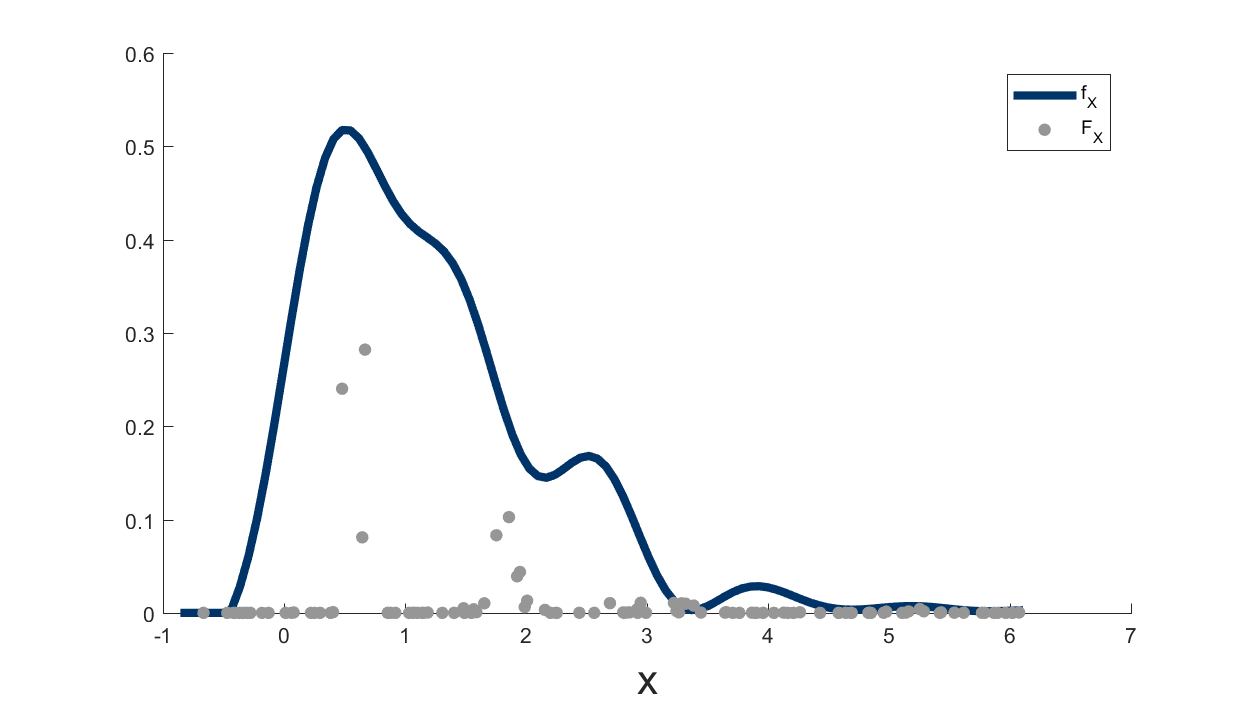
\includegraphics[width = \textwidth]{Figures/Deconvolution/fixed_masses_example.png}
		\caption[A typical example of $F_{\vect{\theta}, \vect{p}}$ being supported on only a few points]{A typical example of $F_{\vect{\theta}, \vect{p}}$ being supported on only a few points. The probability masses $(\theta_j, p_j)$ are represented by grey points, and the resulting estimating density is in dark blue. The true density is a chi-squared density with 3 degrees of freedom, and the errors were normal with variance $\sigma_U^2 = \sigma_X^2 / 5$. There were $n = 500$ samples taken from $W$. The naive density is a kernel density estimator of the $W_j$.}
		\label{fig:fixed masses example alone}
	\end{figure}

	A theoretical justification for this behaviour is hard to obtain. We have made some observations which could be thought of as being in favour of this phenomenon, but mostly we are just pointing out similarities between this problem, and the maximum likelihood mixtures problem of the last chapter. These observations are left until Section \ref{sec:deconvolution observations and results}.

	In this section, we instead explore the phenomenon empirically, and suggest that we might benefit by allowing both the $\theta_j$ and $p_j$ to be the variables of our optimization, rather than fixing the $\theta_j$ as suggested in \cite{Delaigle2016-la}.

	We start by demonstrating the phenomenon using a variety of parameters and distributions. The base example (Figure \ref{fig:fixed masses example alone}) has the following setup:

	\begin{itemize}
		\item The true distribution, $F_X$, is chi-squared with 3 degrees of freedom, rescaled to have variance $\sigma_X = 1$.
		\item The error distribution, $F_U$, is normal.
		\item The noise to signal ratio (NSR) is 1/5. That is, $\sigma_U^2 = \sigma_X^2 / 5$.
		\item We sample $n = 500$ points of $W = X+U$.
	\end{itemize}

	As recommended in the paper, we use $m = 5\sqrt{n}$ point masses in our approximating distribution $\hat{F}_X$. In each of Figures \ref{fig:fixed masses example NSR1}, \ref{fig:fixed masses example Ucauchy}, \ref{fig:fixed masses example n10000}, and \ref{fig:fixed masses example Xgamma}, we change one of these properties and plot the result. Of particular interest in each plot is $\hat{F}_X$ which we represent by placing a grey point at each probability mass. In each of these figures, as well as in the base example in Figure \ref{fig:fixed masses example alone}, we observe that the majority of the probability masses of $\hat{F}_X$ take values very close to, or equal to zero.

	% \begin{figure}
	% 	\centering
	% 	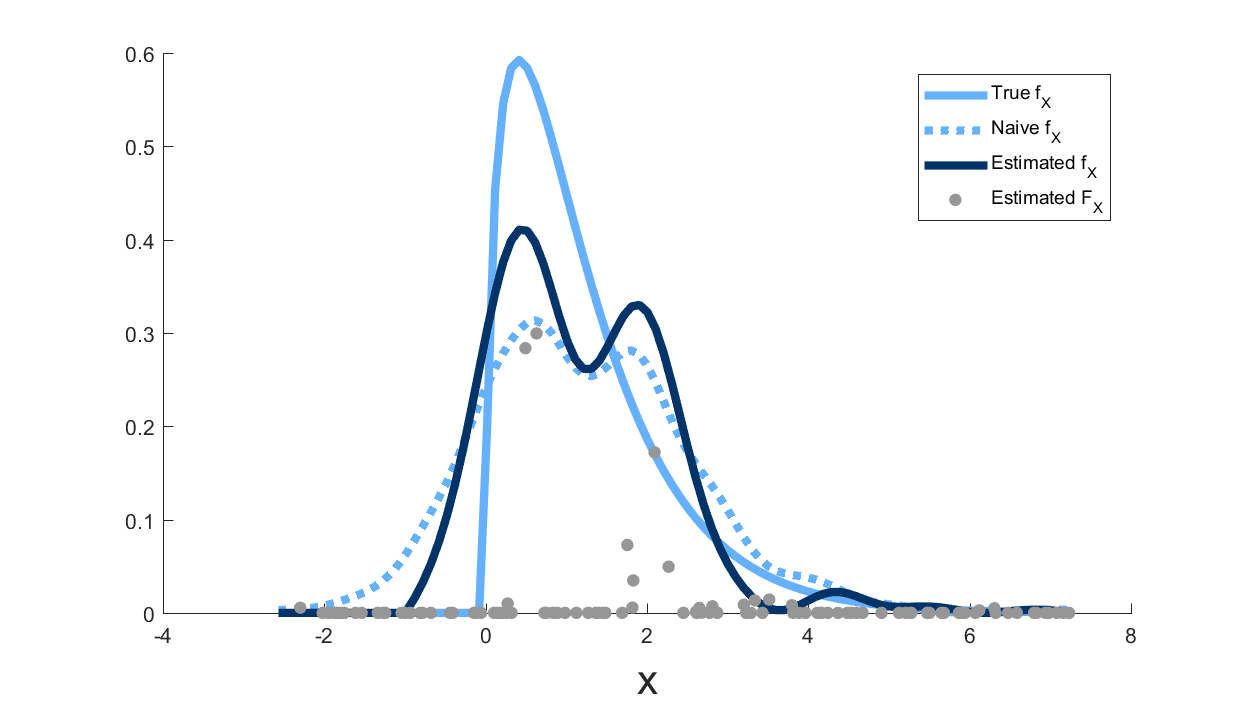
\includegraphics[width = \textwidth]{Figures/Deconvolution/fixed_masses_example_NSR1.png}
	% 	\caption{Blah}
	% 	\label{fig:fixed masses example NSR1}
	% \end{figure}

[REGENERATE THESE FIGURE USING DESKTOP]
\begin{figure}
	\begin{subfigure}[b]{0.49\textwidth}
		\centering
		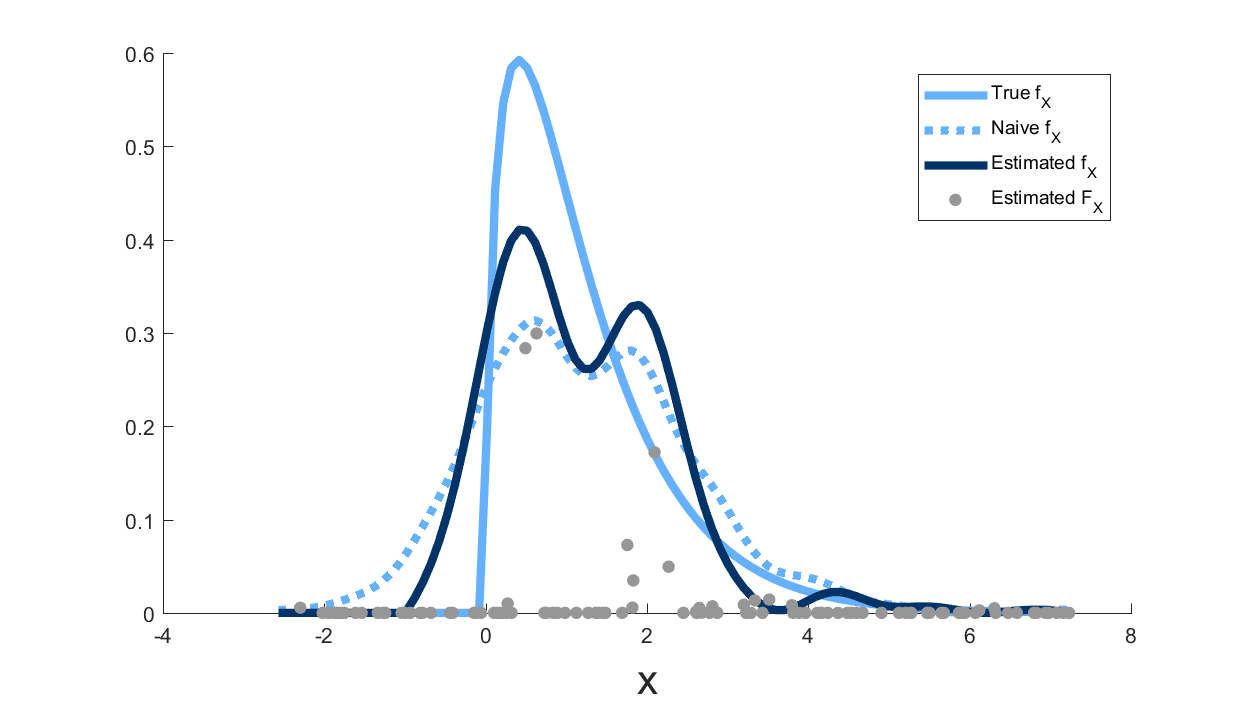
\includegraphics[width = \textwidth]{Figures/Deconvolution/fixed_masses_example_NSR1.png}
		\caption{Using a NSR of 1}
		\label{fig:fixed masses example NSR1}
	\end{subfigure}
	\hfill
	\begin{subfigure}[b]{0.49\textwidth}
		\centering
		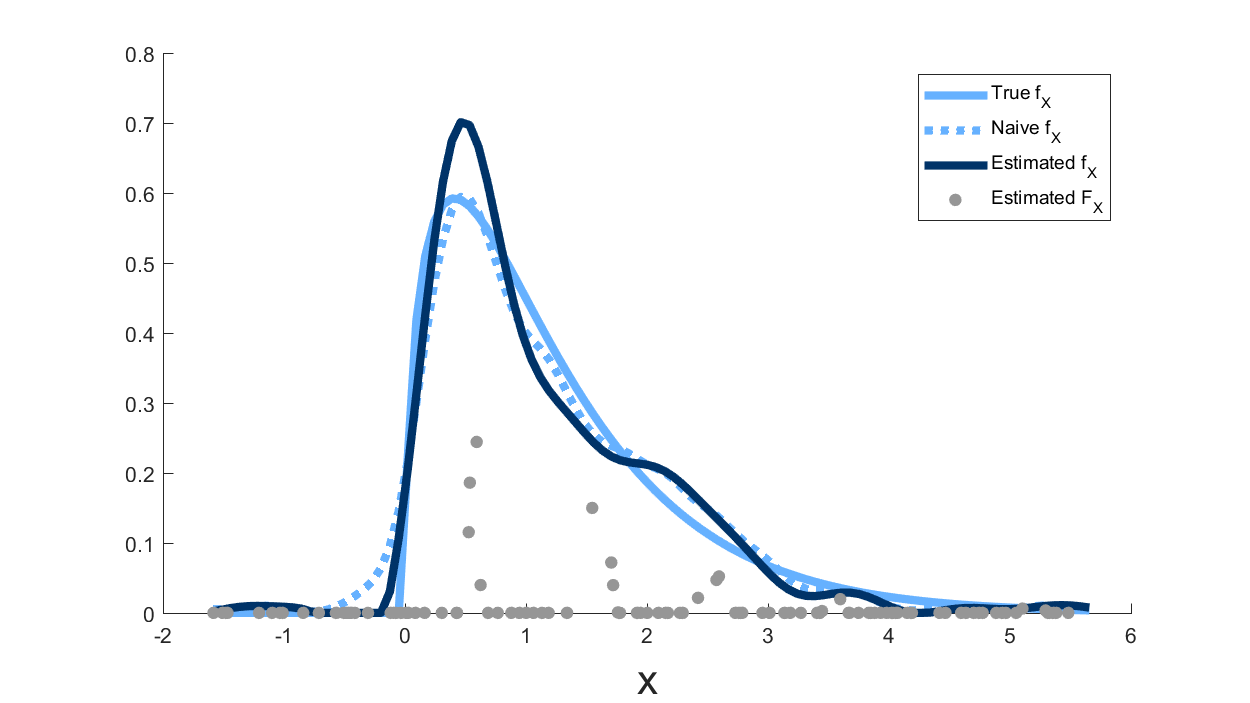
\includegraphics[width = \textwidth]{Figures/Deconvolution/fixed_masses_example_Ucauchy.png}
		\caption{Using a cauchy error distribution}
		\label{fig:fixed masses example Ucauchy}
	\end{subfigure}
	\begin{subfigure}[b]{0.49\textwidth}
		\centering
		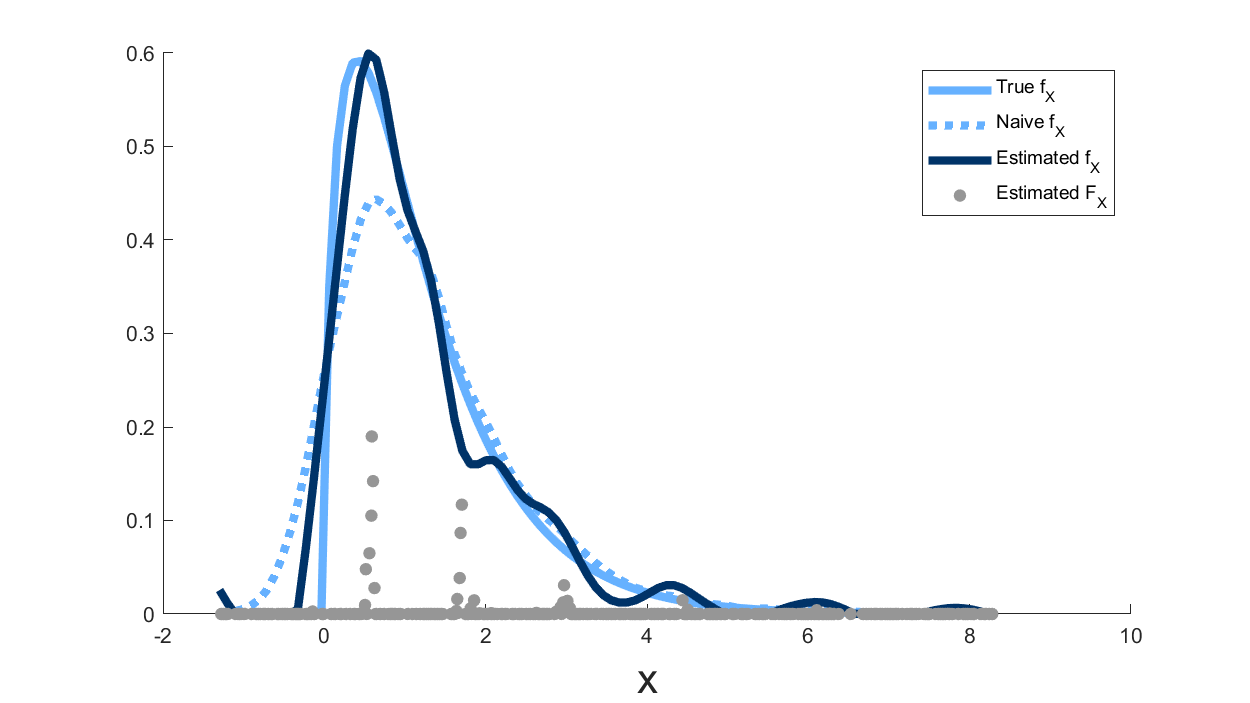
\includegraphics[width = \textwidth]{Figures/Deconvolution/fixed_masses_example_n10000.png}
		\caption{Using $n = 10000$ points}
		\label{fig:fixed masses example n10000}
	\end{subfigure}
	\hfill
	\begin{subfigure}[b]{0.49\textwidth}
		\centering
		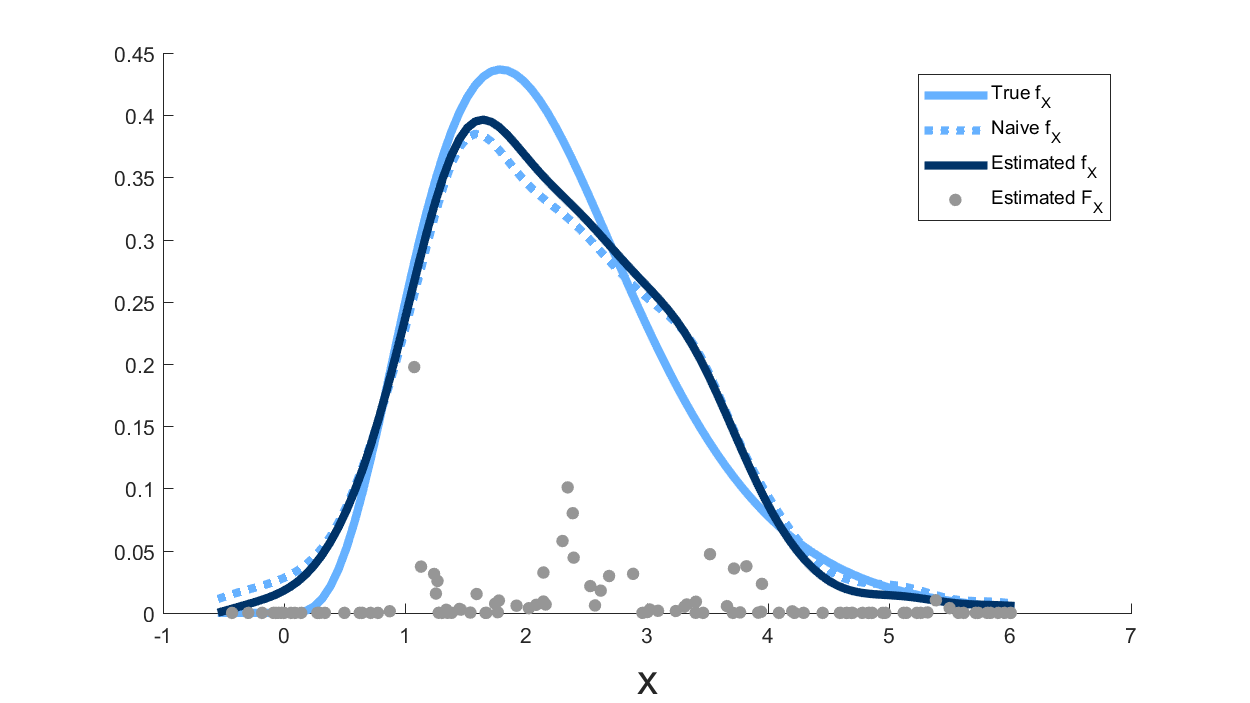
\includegraphics[width = \textwidth]{Figures/Deconvolution/fixed_masses_example_Xgamma.png}
		\caption{Using a gamma(5,2) true distribution}
		\label{fig:fixed masses example Xgamma}
	\end{subfigure}
	\caption{Four variations on the base example in Figure \ref{fig:fixed masses example alone}.}
	\label{fig:comparison different fixed masses examples}
\end{figure}

Given that most of the probability masses of $\hat{F}_X$ do not contribute to the final density, we might hope to reduce the complexity of our optimization problem by using a more appropriate number of masses. Of course, we do not know a priori where these masses should be located along the x axis, and so should make their locations variables in our optimization. This essentially doubles the dimension of our optimization and so to achieve any computational speed up we should aim to use fewer than half the original number of points. In the figures above, we observe that roughly 10 to 20 points out of $m = 112$ or $m = 500$ masses have weights that are visibly greater than 0. Furthermore, it is feasible that two points located close to each other might coalesce into a single point in such a way as to improve the objective if their locations are allowed to vary. This encourages us to proceed using roughly 10 to 20 probability masses with variable weights and locations for $\hat{F}_X$.

\begin{figure}
	\centering
	\begin{subfigure}[b]{0.49\textwidth}
		\centering
		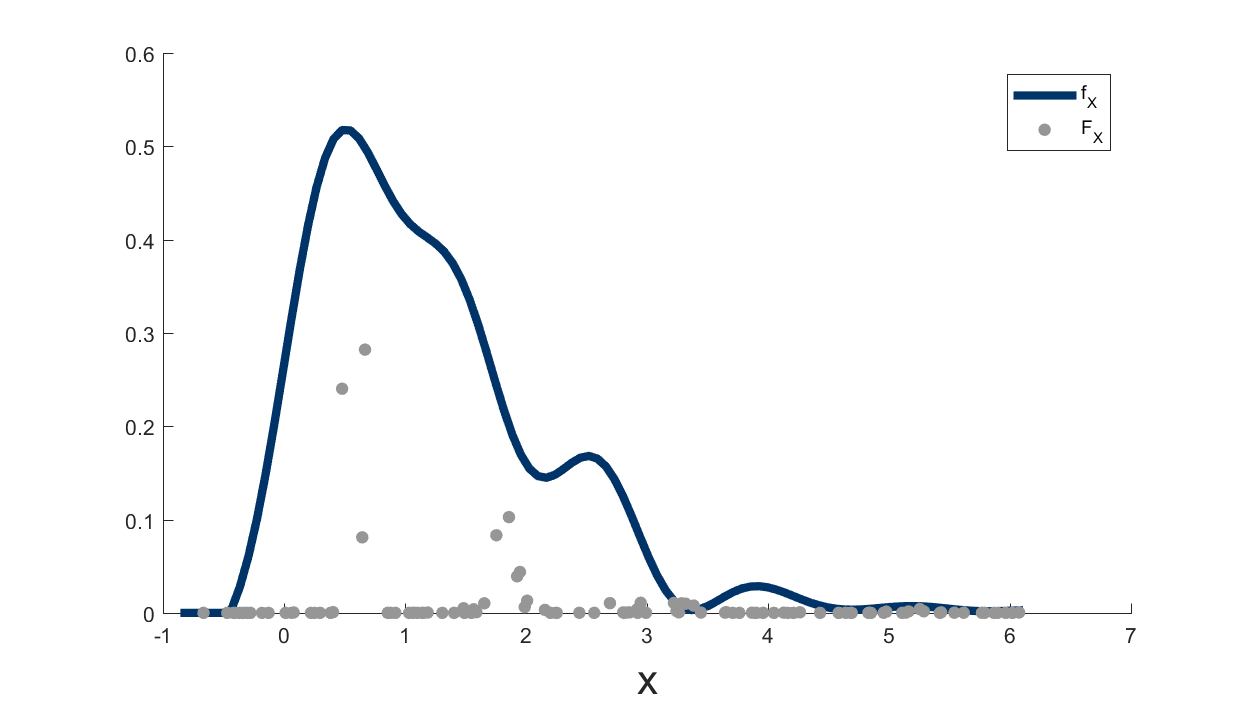
\includegraphics[width = \textwidth]{Figures/Deconvolution/fixed_masses_example.png}
		\begin{tabular}{r l}
			$OBJ_1$ & 0.2284\\
			$\var \hat{F}_X$ & 0.8613\\
			$T(\hat{F}_X)$ & 3.8697e-07\\
			$P1$ & 4.5679e-04\\
			$P2$ & 0\\
			$t$ & 195s
		\end{tabular}
		\caption{112 fixed masses}
		\label{fig:fixed masses example}
	\end{subfigure}
	\hfill
	\begin{subfigure}[b]{0.49\textwidth}
		\centering
		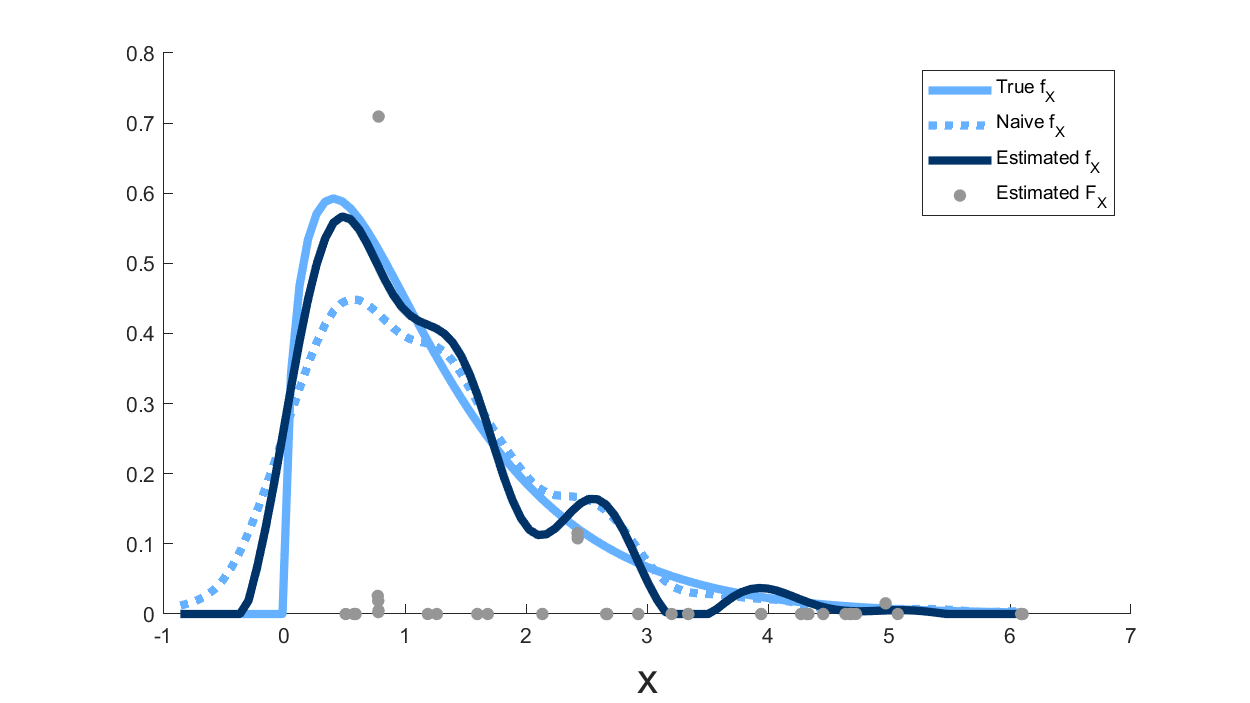
\includegraphics[width = \textwidth]{Figures/Deconvolution/moving_masses_m40_example.png}
		\begin{tabular}{r l}
			$OBJ_1$ & 54.3622\\
			$\var \hat{F}_X$ & 0.6554\\
			$T(\hat{F}_X)$ & 1.7882e-06\\
			$P1$ & 0.1087\\
			$P2$ & 0\\
			$t$ & 76s
		\end{tabular}
		\caption{40 moving masses}
		\label{fig:moving masses m40 example}
	\end{subfigure}
	\begin{subfigure}[b]{0.49\textwidth}
		\centering
		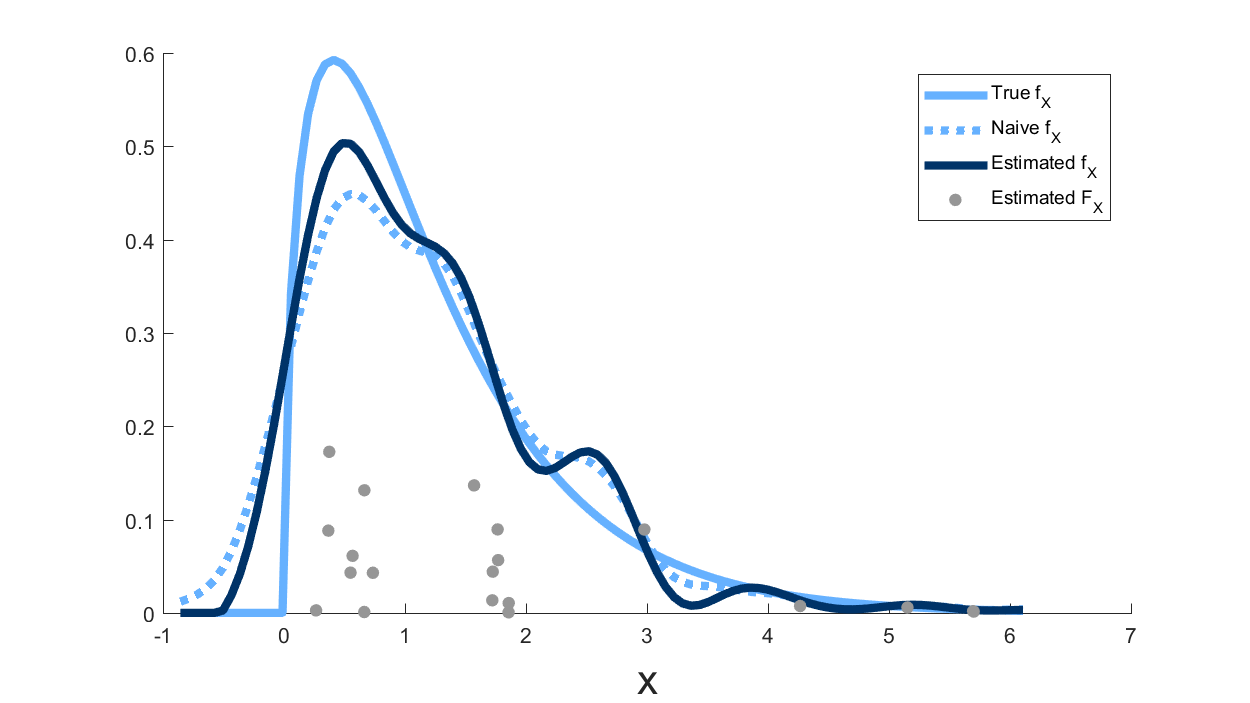
\includegraphics[width = \textwidth]{Figures/Deconvolution/moving_masses_m20_example.png}
		\begin{tabular}{r l}
			$OBJ_1$ & 0.0396\\
			$\var \hat{F}_X$ & 0.8042\\
			$T(\hat{F}_X)$ & 4.4981e-07\\
			$P1$ & 7.9209e-05\\
			$P2$ & 0\\
			$t$ & 37s
		\end{tabular}
		\caption{20 moving masses}
		\label{fig:moving masses m20 example}
	\end{subfigure}
	\hfill
	\begin{subfigure}[b]{0.49\textwidth}
		\centering
		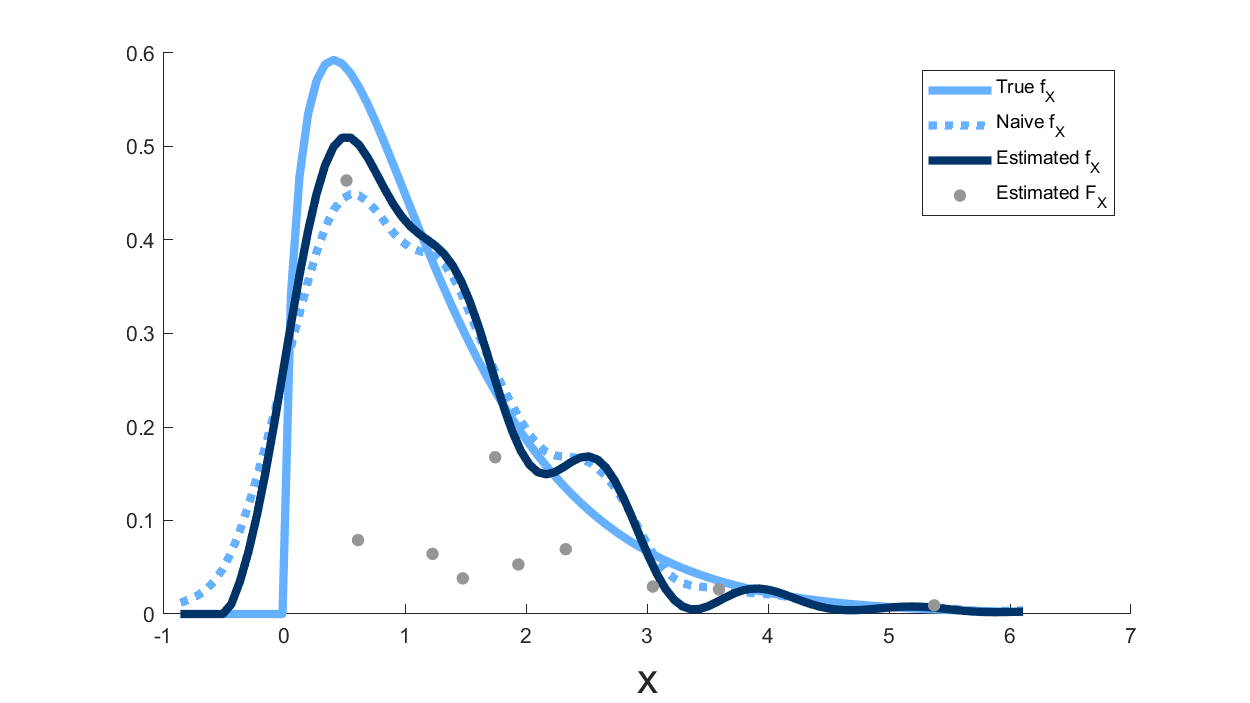
\includegraphics[width = \textwidth]{Figures/Deconvolution/moving_masses_m10_example.png}
		\begin{tabular}{r l}
			$OBJ_1$ & 0.1374\\
			$\var \hat{F}_X$ & 0.8269\\
			$T(\hat{F}_X)$ & 4.2464e-07\\
			$P1$ & 2.7478e-04\\
			$P2$ & 0\\
			$t$ & 15s
		\end{tabular}
		\caption{10 moving masses}
		\label{fig:moving masses m10 example}
	\end{subfigure}
	\begin{subfigure}[b]{0.49\textwidth}
		\centering
		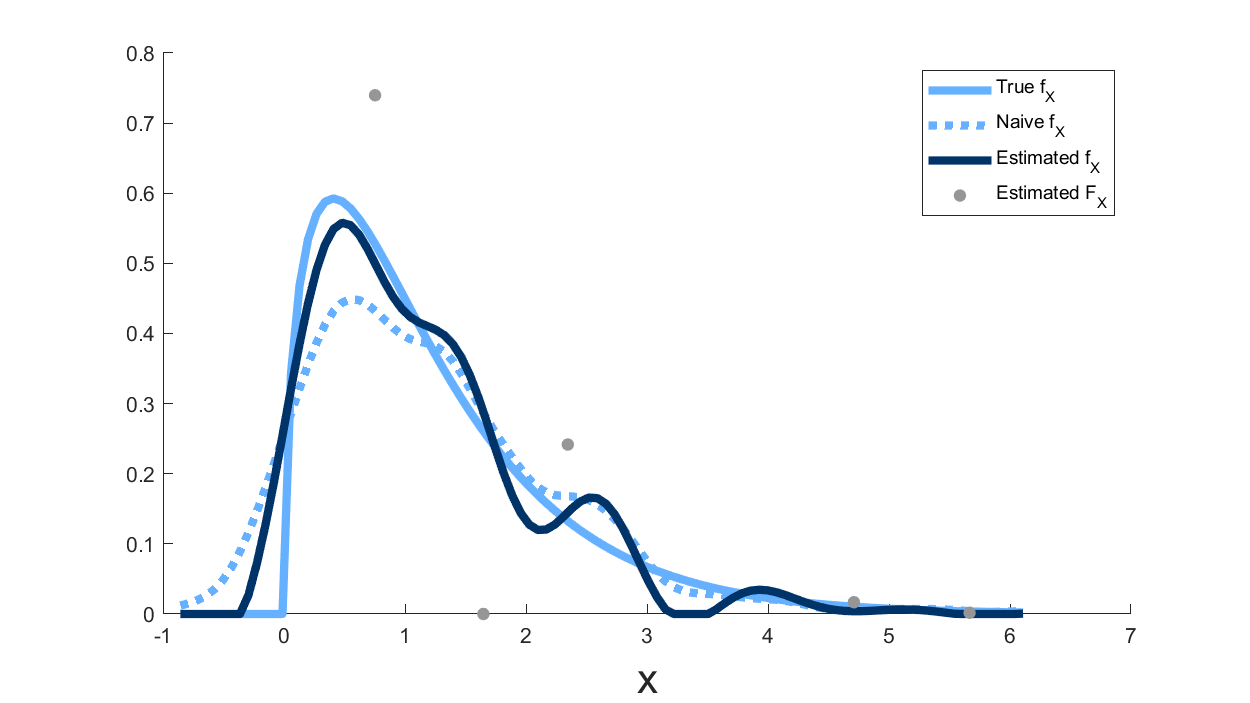
\includegraphics[width = \textwidth]{Figures/Deconvolution/moving_masses_m5_example.png}
		\begin{tabular}{r l}
			$OBJ_1$ & 0.3905\\
			$\var \hat{F}_X$ & 0.8888\\
			$T(\hat{F}_X)$ & 3.6213e-07\\
			$P1$ & 7.8093e-04\\
			$P2$ & 0\\
			$t$ & 4s
		\end{tabular}
		\caption{5 moving masses}
		\label{fig:moving masses m5 example}
	\end{subfigure}
	\hfill
	\begin{subfigure}[b]{0.49\textwidth}
		\centering
		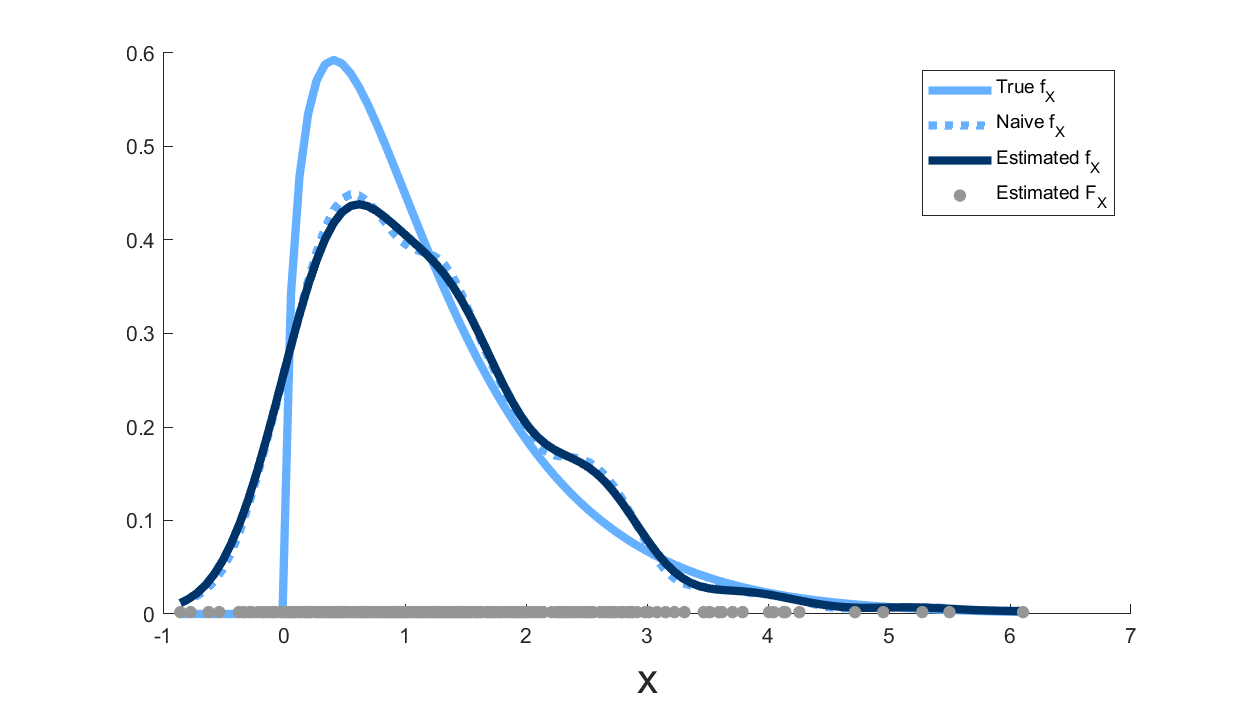
\includegraphics[width = \textwidth]{Figures/Deconvolution/emp_masses_example.png}
		\begin{tabular}{r l}
			$OBJ_1$ & 2.7811e-07\\
			$\var \hat{F}_X$ & 1.0350\\
			$T(\hat{F}_X)$ & 2.7810e-07\\
			$P1$ & 1.0079e-14\\
			$P2$ & 1.7097e-14\\
			$t$ & NA
		\end{tabular}
		\caption{The empirical distribution of W}
		\label{fig:emp masses example}
	\end{subfigure}
	
	\caption{Comparison of results between fixed and variable probability mass locations.}
	\label{fig:compare fixed moving masses}
\end{figure}

We start with Figure \ref{fig:compare fixed moving masses} in which we compare the result we obtain using the fixed masses method of Delaigle and Hall, and the results we obtain when we allow the location of the probability masses in $F_{\vect{\theta}, \vect{p}}$ to vary. As well as plotting $\hat{F}_X$ and $\hat{f}_X$, we also provide a table with the various objective values obtained in the final result, as well as the time taken to run the code on a i5-4670K CPU running at 4.3 GHz, running MATLAB R2018a. For comparison, we also give the various objective values obtained by using the empirical distribution of $W$ as $\hat{F}_X$. The values $T$, $P1$, $P2$ are as defined in Section \ref{sec:deconvolution estimator}, we use $OBJ1$ to denote the objective of our first minimization, $T(F) + \lambda_1 P1(F) + \lambda_2 P2(F)$, and $\var$ to denote the variance of $\hat{F}_X$ (our second objective).

For this particular example, we note that we need only 10 masses to obtain smaller values for both of our objectives when compared to the original fixed masses, and that this results in a significant speed up, as expected. We get even further improvement going from 10 to 20 masses. However, when we use 40 masses, we note that $OBJ_1$ is significantly larger than in any of the cases where we use fewer masses, and that $\var\hat{F}_X$ is smaller than in any other case. One potential explanation here is that the parameter space becomes too complex for our optimization routine to find good solutions if we allow too many moving masses and so $OBJ_1$ is much larger than the global minimum. This means that when we come to our second objective of minimizing $\var \hat{F}_X$, the constraints $T(F) \leq T_\mathrm{min}$, $P1(F) \leq P1_\mathrm{min}$, and $P2(F) \leq P2_\mathrm{min}$ are lax, and so we have more room to search for feasible distributions with small variance.

It also appears as if the 40 mass case is a closer fit for the true curve than any of the other estimates, despite acheiving worse results in the first objective. Although this is purely conjecture, we suggest that this could be because the constraints $T(F) \leq T_\mathrm{min}$, $P1(F) \leq P1_\mathrm{min}$, and $P2(F) \leq P2_\mathrm{min}$ are often too strict to acheive the variance we desire in the second optimization. The first optimization found a solution which just happened to be far enough away from the global minimum to allow for enough freedom in minimizing the variance that we obtained a result that acheived closer to the true variance. One could try using as constraints, $T(F) \leq (1 + \delta) T_\mathrm{min}$, $P1(F) \leq (1 + \delta) P1_\mathrm{min}$, and $P2(F) \leq (1 + \delta) P2_\mathrm{min}$, to allow for this behaviour when the first minimization attains a result closer to the global optimum, but we cannot see any obvious way to determine good values for $\delta$.

The results in Figure \ref{fig:compare fixed moving masses} are encouraging, and in our experience are consistent in a wide variety of scenarios. We present some more examples in Figure \ref{fig:more deconvolution examples}. Of course, it is possible that there is a wide class of deconvolution problems in which a large number of point masses are required to acheive a good solution, and that we have just happened to avoid examples of these. However, we do not think that this is a large concern. One can simply repeat the deconvolution with an increasing number of point masses in $\hat{F}_X$ until it does not result in an improvement in our objectives.

\begin{figure}
	\centering
	\begin{subfigure}[b]{0.4\textwidth}
		\centering
		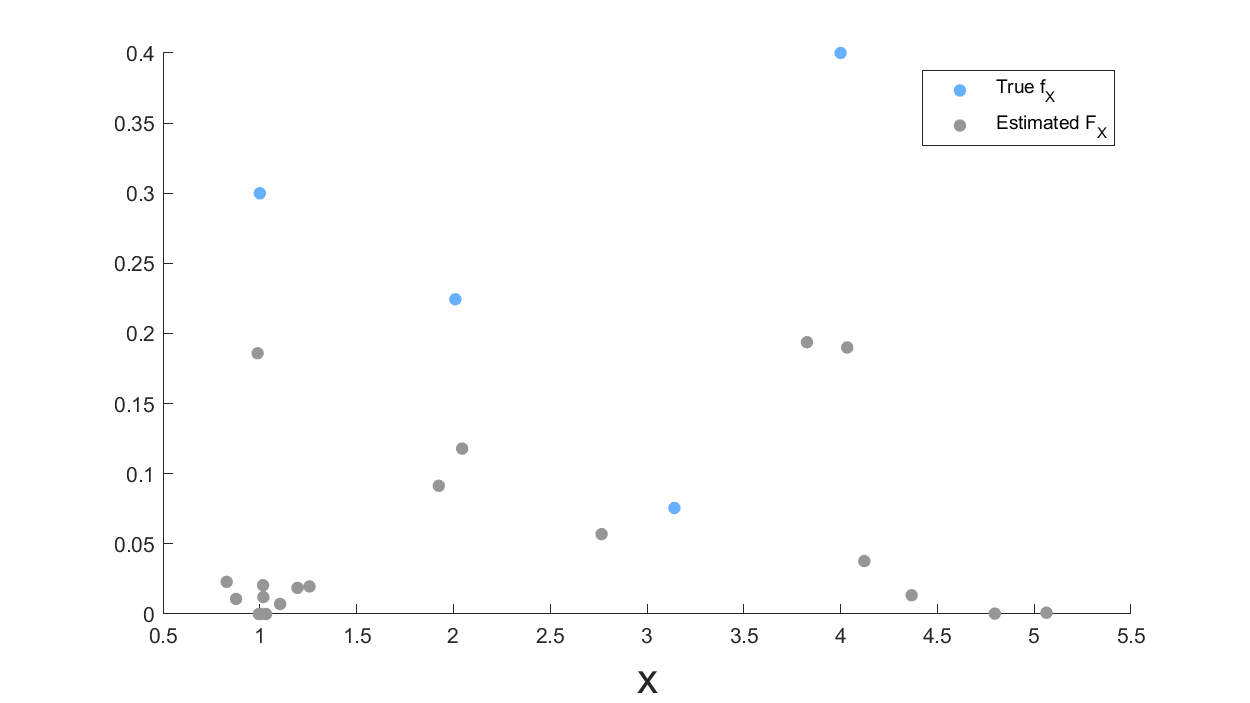
\includegraphics[width = \textwidth]{Figures/Deconvolution/moving_masses_discrete_n5000_example.png}
		\begin{tabular}{r l}
			$OBJ_1$ & 0.8786\\
			$\var \hat{F}_X$ & 1.6542\\
			$T(\hat{F}_X)$ & 1.1094e-08\\
			$P1$ & 0.0018\\
			$P2$ & 0\\
			$t$ & 62s
		\end{tabular}
		\caption{True distribution discrete (represented by blue points) with normal errors, $n = 5000$, moving masses.}
		\label{fig:moving masses discrete}
	\end{subfigure}
	\hfill
	\begin{subfigure}[b]{0.4\textwidth}
		\centering
		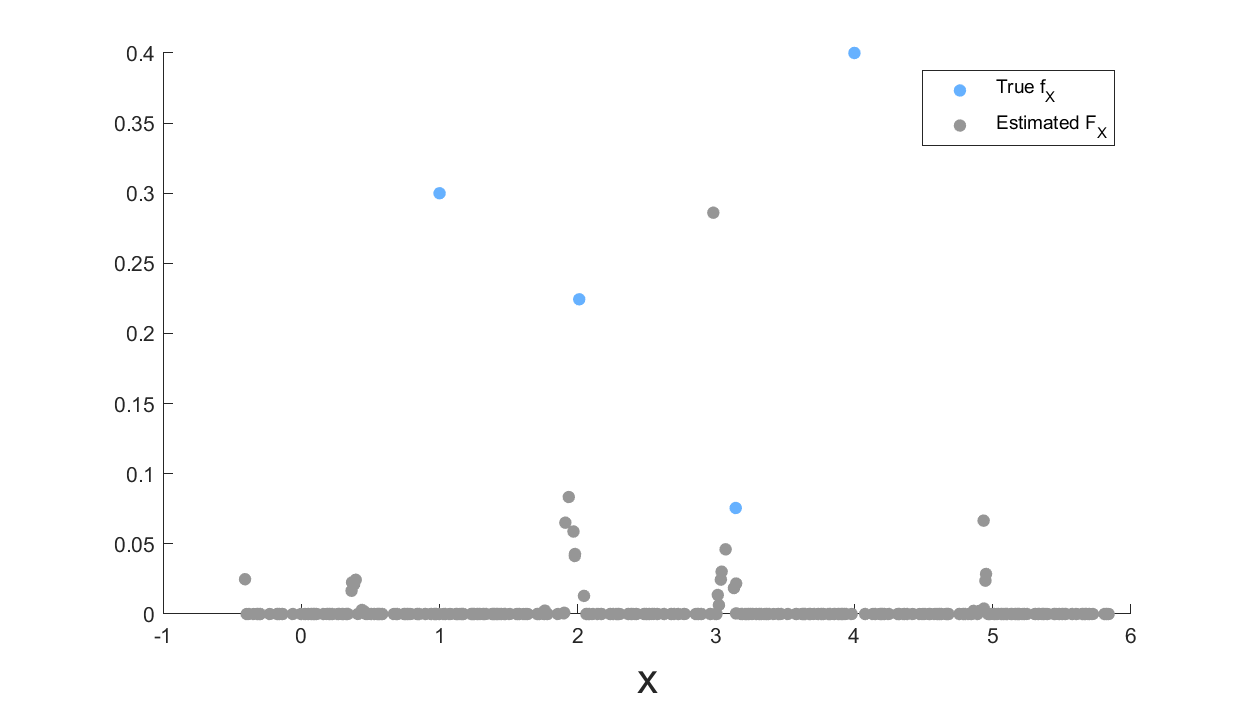
\includegraphics[width = \textwidth]{Figures/Deconvolution/fixed_masses_discrete_n5000_example.png}
		\begin{tabular}{r l}
			$OBJ_1$ & 106.6533\\
			$\var \hat{F}_X$ & 1.5731\\
			$T(\hat{F}_X)$ & 0.0192\\
			$P1$ & 0.2133\\
			$P2$ & 0\\
			$t$ & 1354s
		\end{tabular}
		\caption{True distribution discrete (represented by blue points) with normal errors, $n = 5000$, fixed masses.}
		\label{fig:fixed masses discrete}
	\end{subfigure}
	\begin{subfigure}[b]{0.4\textwidth}
		\centering
		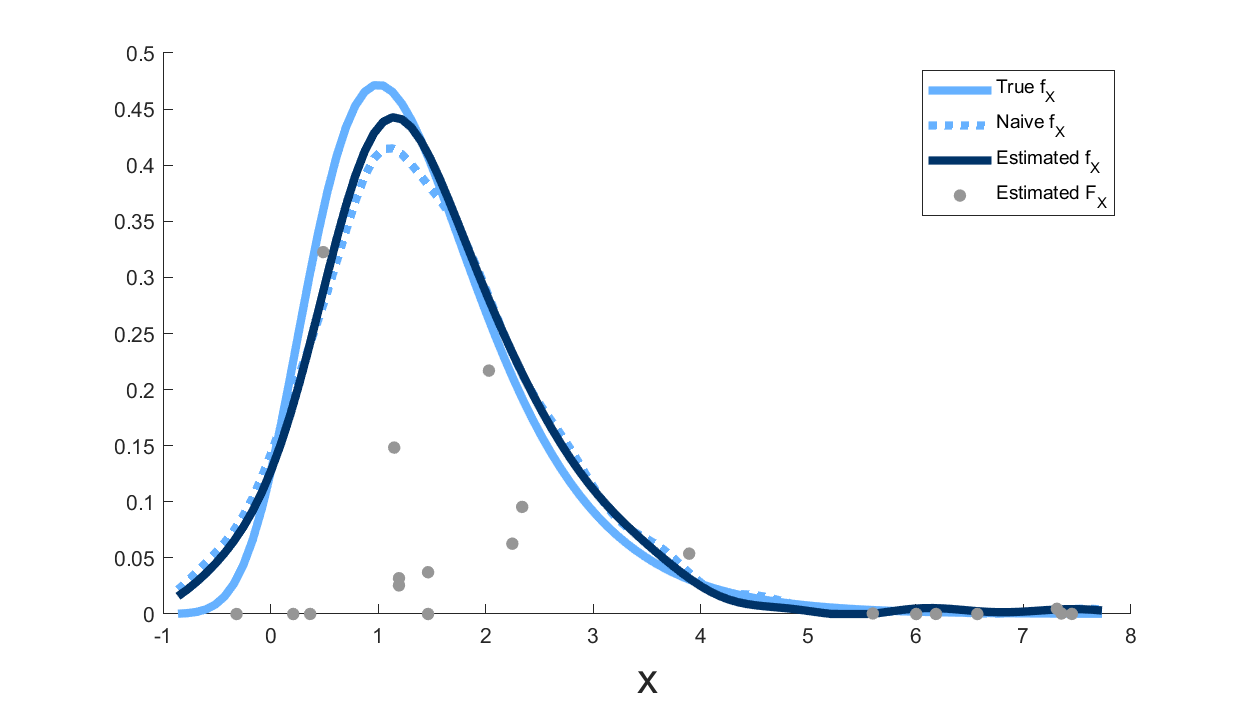
\includegraphics[width = \textwidth]{Figures/Deconvolution/moving_masses_gumbel_lap_example.png}
		\begin{tabular}{r l}
			$OBJ_1$ & 0.3742\\
			$\var \hat{F}_X$ & 1.0063\\
			$T(\hat{F}_X)$ & 3.5329e-07\\
			$P1$ & 7.4839e-04\\
			$P2$ & 0\\
			$t$ & 64s
		\end{tabular}
		\caption{True distribution gumbel with laplace errors, $n = 500$, moving masses.}
		\label{fig:moving masses gumbel lap}
	\end{subfigure}
	\hfill
	\begin{subfigure}[b]{0.4\textwidth}
		\centering
		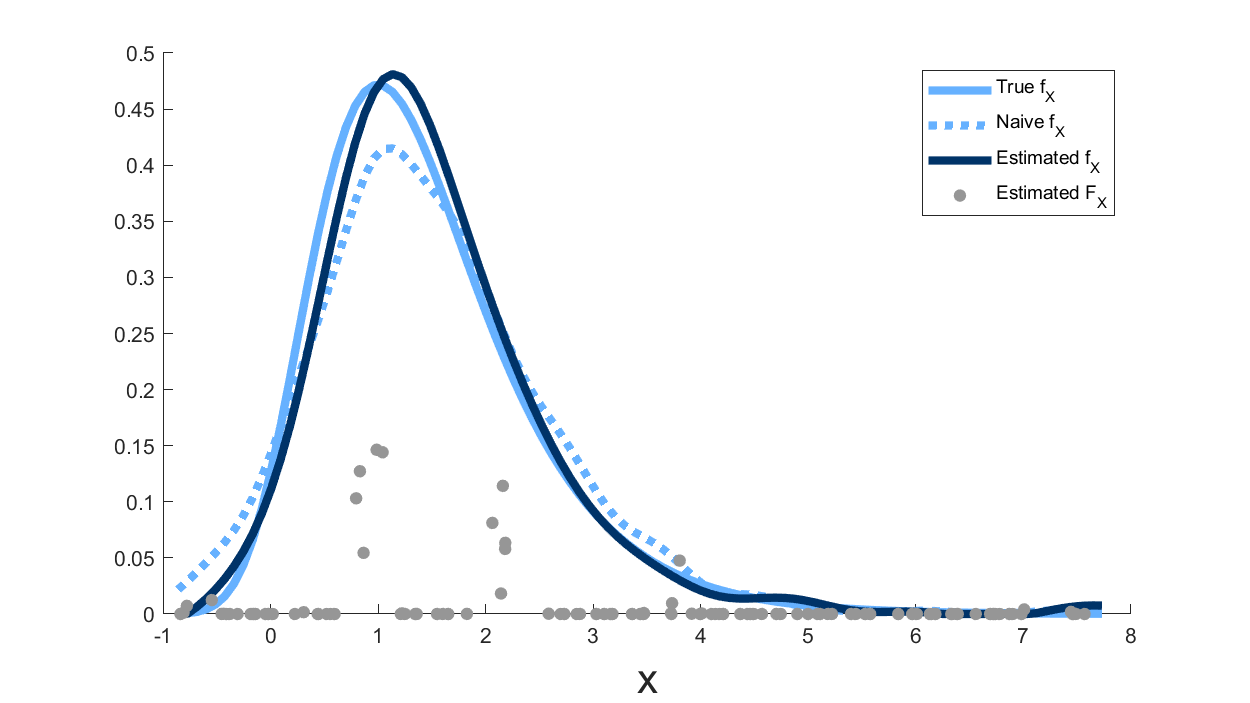
\includegraphics[width = \textwidth]{Figures/Deconvolution/fixed_masses_gumbel_lap_example.png}
		\begin{tabular}{r l}
			$OBJ_1$ & 0.2603\\
			$\var \hat{F}_X$ & 0.9413\\
			$T(\hat{F}_X)$ & 4.9281e-07\\
			$P1$ & 5.2056e-04\\
			$P2$ & 0\\
			$t$ & 195s
		\end{tabular}
		\caption{True distribution gumbel with laplace errors, $n = 500$, fixed masses.}
		\label{fig:fixed masses gumbel lap}
	\end{subfigure}
	\begin{subfigure}[b]{0.4\textwidth}
		\centering
		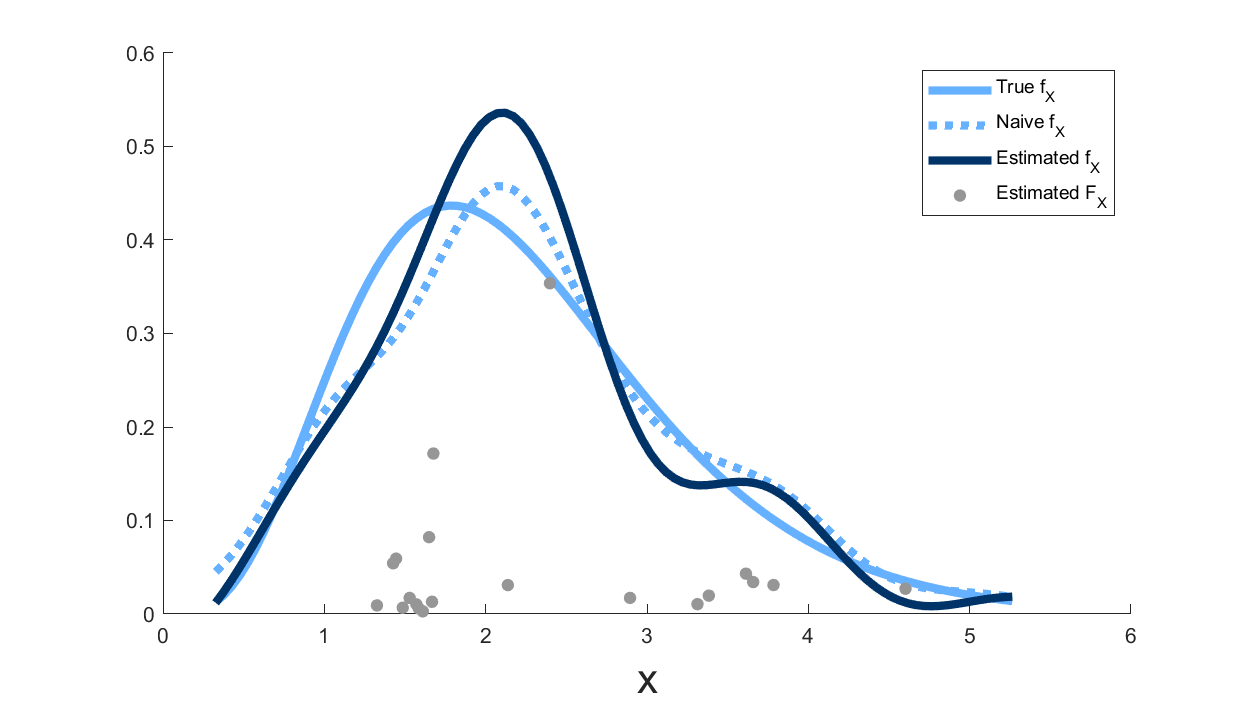
\includegraphics[width = \textwidth]{Figures/Deconvolution/moving_masses_gamma_discrete_n100_example.png}
		\begin{tabular}{r l}
			$OBJ_1$ & 0.1506\\
			$\var \hat{F}_X$ & 0.6176\\
			$T(\hat{F}_X)$ & 1.2286e-05\\
			$P1$ & 3.0108e-04\\
			$P2$ & 0\\
			$t$ & 47s
		\end{tabular}
		\caption{True distribution Gamma(5,2), with errors discrete (-1,0,1) with probabilities (0.2,0.6,0.2), $n = 100$, moving masses.}
		\label{fig:moving masses gamma discrete}
	\end{subfigure}
	\hfill
	\begin{subfigure}[b]{0.4\textwidth}
		\centering
		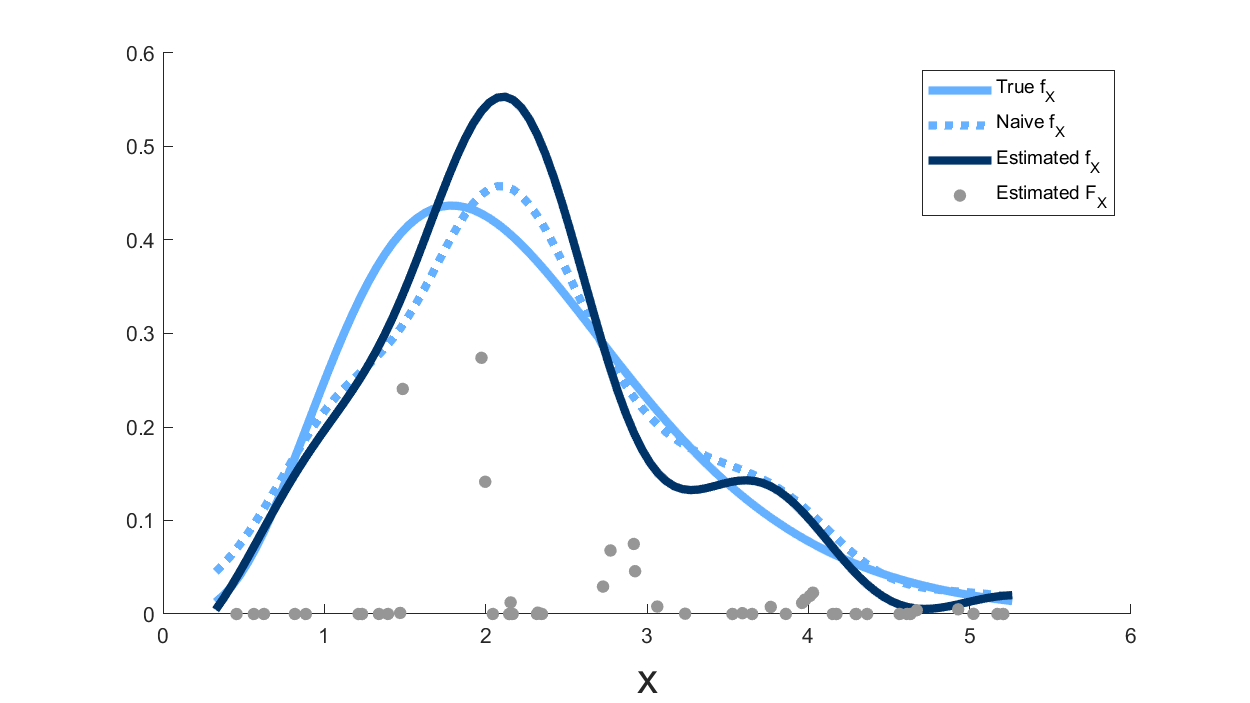
\includegraphics[width = \textwidth]{Figures/Deconvolution/fixed_masses_gamma_discrete_n100_example.png}
		\begin{tabular}{r l}
			$OBJ_1$ & 0.1681\\
			$\var \hat{F}_X$ & 0.5953\\
			$T(\hat{F}_X)$ & 1.2921e-05\\
			$P1$ & 3.3615e-04\\
			$P2$ & 0\\
			$t$ & 62s
		\end{tabular}
		\caption{True distribution Gamma(5,2), with errors discrete (-1,0,1) with probabilities (0.2,0.6,0.2), $n = 100$, fixed masses.}
		\label{fig:fixed masses gamma discrete}
	\end{subfigure}
	\caption{Three more comparisons between moving masses and fixed masses.}
	\label{fig:more deconvolution examples}
	\end{figure}

\subsection{R Package}
Given all the discussion above, we see no reason not to use masses with variable locations. We have used this new method in the R Package `deconvolve'

[UP TO HERE]

[PUT IN TIME COMPARISONS HERE]

% \begin{figure}
% 	\centering
% 	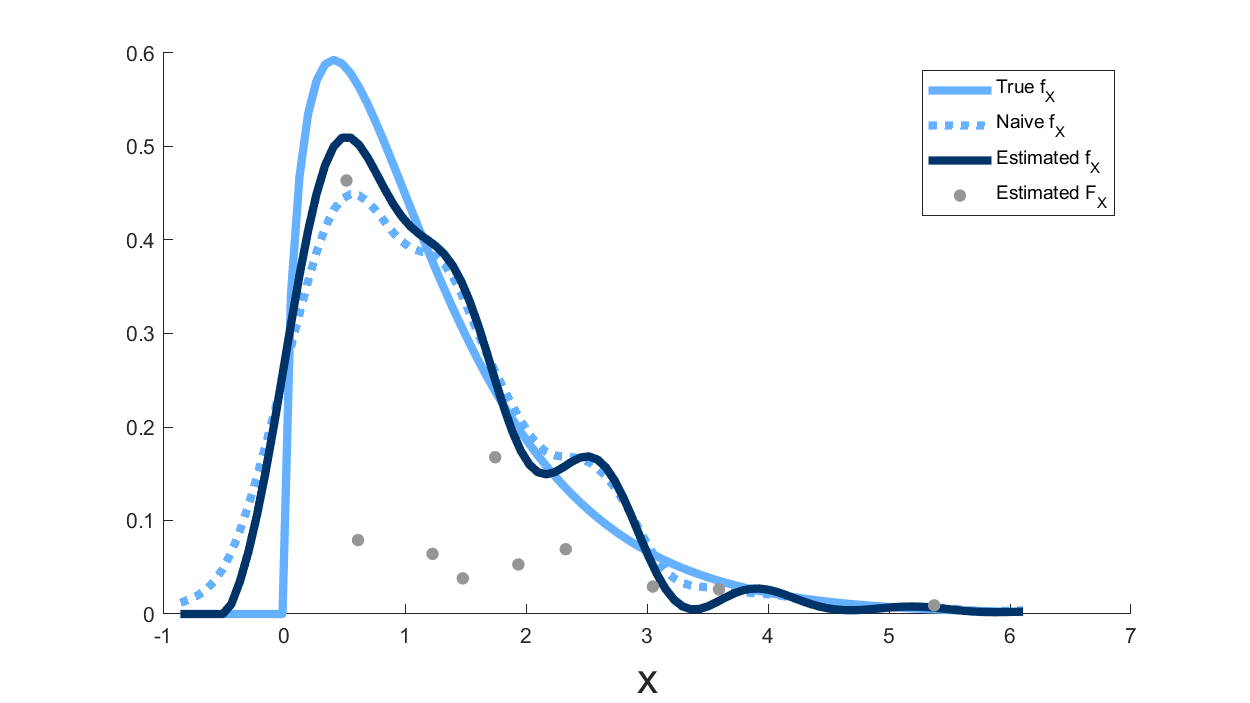
\includegraphics[width = \textwidth]{Figures/Deconvolution/moving_masses_m10_example.png}
% 	\begin{tabular}{r l}
% 		$\var \hat{F}_X$ & 0.9011\\
% 		$T(\hat{F}_X)$ & 3.5540e-07\\
% 		$P1$ & 7.0136e-05\\
% 		$P2$ & 0\\
% 		$t$ & 492
% 	\end{tabular}
% 	\caption{blah}
% 	\label{fig:moving masses m10 example}
% \end{figure}



\subsection{No penalties seems to make behaviour stronger}

\subsection{Discrete X?}

	

\section{General Observations and Results}
\label{sec:deconvolution observations and results}

We end this section with two simple observations about our deconvolution problem. We do not claim that either of these theorems are new, but we think that they are still worth stating.
We start with the observation that the set of distributions with equal phase function is a convex set.

	% \subsection{Results concerning phase functions}
	\begin{theorem}
	\label{thm:equal phase functions convex set}
		Let $F_X$ and $F_Y$ be two distributions, and let
		\begin{align}
			F_Z &= (1 - \lambda) F_X + \lambda F_Y && \lambda \in [0,1]
		\end{align}
		be a convex combination of these distributions. If $\rho_X = \rho_Y$, then 
		\begin{equation}
			\rho_Z = \rho_X = \rho_Y.
		\end{equation}
	\end{theorem}
	\begin{proof}
		Write $\phi_X$ and $\phi_Y$ for the characteristic functions of $X$ and $Y$. These are complex valued functions which we can write in the form
		\begin{align}
			\phi_X &= r_X(t) \euler^{i\theta_X(t)},\\
			\phi_Y &= r_Y(t) \euler^{i\theta_Y(t)},
		\end{align}
		where $r_X(t), r_Y(t)$ take values on $[0, 1]$ and where
		\begin{align}
			\rho_X &= \euler^{i\theta_X(t)},\\
			\rho_Y &= \euler^{i\theta_Y(t)}.
		\end{align}
		The characteristic function of $F_Z$ is 
		\begin{align}
			\phi_Z &= \int \euler^{itx} \intd \left[(1 - \lambda)F_X(x) + \lambda F_Y(x)\right]\\
			&= (1 - \lambda)\phi_X + \lambda \phi_Y\\
			&= (1 - \lambda) r_X(t) \rho_X + \lambda r_Y(t) \rho_Y.
		\end{align}

		If $\rho_X = \rho_Y$ then
		\begin{equation}
			\phi_Z = \left((1 - \lambda)r_X(t) + \lambda r_Y(t)\right) \rho_X
		\end{equation}
		and so 
		\begin{equation}
			\rho_Z = \rho_X = \rho_Y.
		\end{equation}
	\end{proof}

Recall that ideally, we would like to search the set of all distributions with phase function equal to that of $W$ to find the distribution with smallest variance. Theorem \ref{thm:equal phase functions convex set} tells us that this set is convex. Furthermore, given any two distributions $F_X$ and $F_Y$ with variances $\sigma_X^2$ and $\sigma_Y^2$ respectively, a convex combination of them, $F_Z = (1 - \lambda)F_X + \lambda F_Y$, will have variance $\sigma_Z^2 \geq (1 - \lambda) \sigma_X^2 + \lambda \sigma_Y^2$.

[UP TO HERE AS WELL]

[VARIANCE IS CONCAVE]

	% TESTING
	% \begin{proof}
	% 	\begin{align}
	% 		|\rho_Z - \rho_W| &= \left| \frac{(1 - \lambda)\phi_X + \lambda \phi_Y}{|(1 - \lambda)\phi_X + \lambda \phi_Y|} - \rho_W \right|\\
	% 		&= \left| \frac{(1 - \lambda)\phi_X + \lambda \phi_Y - |(1 - \lambda)\phi_X + \lambda \phi_Y| \rho_W}{|(1 - \lambda)\phi_X + \lambda \phi_Y|}\right|
	% 	\end{align}

	% 	\begin{align}
	% 		\phi_Z &= (1 - \lambda) r_X \rho_X + \lambda r_Y \rho_Y\\
	% 		|\phi_Z| &\leq (1 - \lambda) r_X + \lambda r_Y\\
	% 		\phi_Z &= (1 - \lambda) r_X \rho_X + \lambda r_Y \rho_X + \lambda r_Y (\rho_Y - \rho_X)\\
	% 	\end{align}
	% \end{proof}

% \subsection{A particular class of optimization problem}
		"The results follow from this general theorem which seems obvious."

		\begin{theorem}
			\label{thm:solution in interior}
			Let $(E_m)_{m=1}^\infty$ be a sequence of appropriately defined sets and let
			$(g_m)_{m=1}^\infty, g_m: E_m \mapsto \mathbb{R}$ be a sequence of
			functions that satisfy the following properties
			\begin{enumerate}
				\item $\forall \vect{x} \in \partial E_m, \exists n < m, \vect{y} \in E_n$ such that
				$g_m(\vect{x}) \leq g_n(\vect{y})$.
				\label{prop:one}
				\item $\exists m_0, \vect{x}_0 \in E_{m_0}$ such that $\forall m, \vect{x} \in 
				E_m$, $g_m(\vect{x}) \leq g_{m_0}(\vect{x}_0)$.
			\end{enumerate}
			Then $\exists m_*, \vect{x}_* \in E_{m_*} \setminus \partial E_{m_*}$ such
			that $\forall m, \vect{x} \in E_m$, $g_m(\vect{x}) \leq g_{m_*}(\vect{x}_*)$.
		\end{theorem}
		\begin{proof}
			The proof is simple. If $\vect{x}_0 \notin \partial E_{m_0}$ then we are done.
			Otherwise, by property \ref{prop:one} we can find a $n$ and $\vect{y} \in 
			E_n$ such that $g_n(y) = g_{m_0}(\vect{x}_0)$. If $\vect{y} \notin \partial 
			E_n$ then we are done, otherwise we repeat the process until we find a $m, 
			\vect{x}$ pair with $\vect{x} \notin \partial E_m$. %Note that property 
			% \ref{prop:one} implies that $\partial E_1 = \emptyset$ and so this process
			% must end.
		\end{proof}

\section{R Package}